% Internal paper outline, prepared from repository evidence on 14 November 2026.
% This is a planning document, not a submission-ready research manuscript.
% Numerical tables are generated by build_evidence.py from tracked per-source CSVs.
\documentclass[runningheads]{llncs}
\usepackage[utf8]{inputenc}
\usepackage{amsmath,amssymb,graphicx,booktabs,tabularx,tikz,url}
\usepackage[hidelinks]{hyperref}
\pdfstringdefDisableCommands{\def\\{ }\def\large{}}
\usetikzlibrary{arrows.meta,positioning}
\setlength{\tabcolsep}{4pt}
\setlength{\emergencystretch}{2em}
\newcommand{\status}[1]{\textbf{#1}}
\newcommand{\pathref}[1]{\par\noindent{\scriptsize\path{#1}}\par}
\begin{document}
\title{Validation-Data Allocation and Calibration in Diverse Prototypical Ensembles on Waterbirds\\[3pt]
\large ACIIDS 2027: Evidence-Based Paper Outline}
\titlerunning{ACIIDS 2027: Evidence-Based Paper Outline}
\author{Chau Tan Phat\inst{1,2} \and Nguyen Dang Khang\inst{1,2} \and
Nguyen Phu Trong\inst{1,2} \and Nguyen Dinh Minh Huy\inst{1,2}}
\authorrunning{C. T. Phat et al.}
\institute{Faculty of Information Technology, University of Science, Ho Chi Minh City, Vietnam \and
Vietnam National University, Ho Chi Minh City, Vietnam\\
\email{ctphat2519@apcs.fitus.edu.vn, ndkhang2535@apcs.fitus.edu.vn}\\
\email{nptrong2530@apcs.fitus.edu.vn, ndmhuy2521@apcs.fitus.edu.vn}}
\maketitle
\noindent\textbf{Internal planning version: 14 November 2026.} Completed results, unresolved provenance, and proposed work are identified separately throughout. No new Waterbirds model was trained for this outline.

\section{Recommended Framing and Titles}
\textbf{Recommendation: an empirical study with a limited methodological component.}
The strongest question is how to allocate a small adaptation set between learning prototype heads and fitting their final decision rule. The completed experiments show allocation sensitivity and different behavior under two backbone recipes. They do not establish a generally better aggregator. Cross-fitting belongs as an evaluated strategy and a possible extension, rather than the title-level claim of a successful new method.

A purely methodological paper is currently difficult to defend. Cross-fitting, stacking, affine calibration, and threshold selection are established ideas. More importantly, the completed five-fold experiment does not demonstrate that affine calibration improves the original fold ensemble on standard ERM. Reproduction provides the experimental foundation; it is not the contribution.

\textbf{Preferred title.} \emph{Validation-Data Allocation and Calibration in Diverse Prototypical Ensembles on Waterbirds.}
Other defensible options are:
\begin{enumerate}
\item \emph{An Empirical Study of Validation-Data Efficiency in Prototype Ensembles.}
\item \emph{When Does Learned Aggregation Help Prototype Ensembles? Evidence from Waterbirds.}
\item \emph{Prototype Learning or Calibration? Allocation Trade-offs on Waterbirds.}
\item \emph{Cross-Fitting and Decision Calibration for Prototype Ensembles: A Waterbirds Case Study.}
\end{enumerate}
Use the final option only if the cross-fitting protocol and essential calibration controls are fully documented. Avoid claims of state-of-the-art performance, elimination of background shortcuts, or a novel calibration principle.


\section{Evidence Audit: What the Records Actually Establish}
The current ACIIDS folder contained a copy of the Week 2 progress report. Its qualitative viewer, rotation screenshots, and image fusion example do not answer the proposed research question. They should not occupy the paper's main experimental space.

\subsection{A Material Update to the Research Brief}
The independent-methods records contain a completed \emph{five-fold} cross-fitting study [R3], beyond the evidence summarized in the brief. Its inference rule retains five fold ensembles and calibrates each before averaging. This differs from the proposed procedure that transfers a calibrator to one DPE refitted on all 1,199 validation images. The latter remains \status{pending verification/evaluation}. A completed fold-ensemble experiment cannot establish the proposed refit's performance.

\begin{table}[ht]
\centering\small
\caption{Recomputed exploratory test results from [R3]. WGA is mean $\pm$ sample SD across five standard-ERM or two ERM$^*$ sources; OA is mean overall accuracy. All entries are percentages. P0 uses 720/479 images. The four original-head cross-fitted affine settings are all shown, without selecting a test winner.}
\label{tab:evidence}
\input{evidence_table.tex}
\end{table}

The full-validation standard-ERM result is 89.5950\%, versus 91.0\% reported by DPE: a 1.4050 pp gap. ERM$^*$ reaches 94.0810\%, close to the reported 94.1\% \cite{dpe}. These are different training recipes (100 versus 400 backbone epochs), not seven repetitions of one configuration.

For the original-head fold ensemble, all four tested affine means are below uncalibrated standard ERM. For ERM$^*$ they improve on the fold control but remain below full-validation DPE. The uncalibrated standard-ERM fold gain over full-validation DPE is +0.5443 pp; its paired source-level 95\% $t$ interval is [$-0.3726$, +1.4611] pp. This descriptive interval ignores historical selection and repeated test inspection. ERM$^*$ has only two sources: show both source results and avoid population-level inference.

The reported ``+0.47 pp cross-fitting gain'' has no identified matching protocol here. A nearby +0.4730 pp result in earlier records concerns \emph{three-source dropout aggregation}, not verified five-source cross-fitting. Do not equate those claims or place the unverified number in the abstract.


\section{Research Questions, Contributions, and Abstract}
\textbf{RQ1:} How much do conclusions about learned aggregation change when the reference is a matched reduced-data DPE versus a DPE fitted on the full adaptation set?\par
\textbf{RQ2:} Are observed effects stable across validation allocations and the two backbone training recipes?\par
\textbf{RQ3:} Does cross-fitting add value beyond fold ensembling and a validation-selected decision threshold under the same annotation budget?

\subsection{Contributions That Can Be Defended}
\begin{enumerate}
\item \textbf{Controlled characterization:} separate aggregation gains from the cost of reserving adaptation images, using both matched-split and full-validation references. Existing results support allocation sensitivity; they do not isolate a pure causal effect of sample count because update budgets and selection pools also differ.
\item \textbf{Backbone-dependent empirical findings:} document why a fixed residual or weighting procedure can help standard ERM yet fail to transfer to ERM$^*$. Report negative ablations without presenting an exploratory winner as confirmed.
\item \textbf{Cross-fitting analysis:} distinguish fold-ensemble averaging, scalar calibration, and transfer to a full-data refit. Claim an effective adaptation only if the missing controls support it; otherwise report its limits.
\end{enumerate}
The breadth of a sweep and agreement with published baselines do not constitute novelty. The contribution must be the controlled question, evidence, and resulting guidance. The literature gap should be phrased narrowly: an allocation issue in this DPE adaptation pipeline, not a claim that prior work never studied validation efficiency.

\subsection{Abstract Structure}
Use about 160--200 words, with five functions: (1) establish subpopulation robustness and the need for adaptation data; (2) identify competition between prototype fitting and downstream calibration; (3) describe a frozen-feature comparison with full-data and matched-split controls; (4) report verified allocation/backbone sensitivity and the actual status of cross-fitting; (5) conclude with bounded practical guidance. Insert final threshold/DFR findings only after they exist.

\textbf{Evidence-safe working abstract.}
Prototype ensembles adapt frozen representations to subpopulation shift, but adding a learned aggregation layer divides the limited data available for adaptation. We study this allocation problem for Diverse Prototypical Ensembles on Waterbirds using five standard-ERM backbone sources and two sources from an enhanced ERM recipe. We compare full-validation uniform ensembles, fixed-split aggregation, and a five-fold ensemble with out-of-fold affine calibration. Existing exploratory results show that improvements over a reduced-data uniform baseline depend on the validation partition and backbone recipe. Full-validation DPE reaches 89.60\% and 94.08\% mean worst-group accuracy in the two settings. The uncalibrated fold ensemble reaches 90.14\% and 93.60\%, respectively; tested original-head affine variants do not improve its standard-ERM mean, and the standard-ERM fold gain over full-validation DPE has a source-level interval including zero. These observations motivate evaluating data allocation and simple decision controls together. They do not establish a general calibration advantage or reduced causal background reliance. Comparisons with validation-selected thresholds and same-feature last-layer retraining remain necessary before stronger practical recommendations.

\noindent This abstract describes the current study status; remove planning language and add completed essential controls before submission.


\section{Proposed Springer Paper: Section-by-Section Outline}
Target a focused 13--14-page full manuscript including references. This outline itself is an internal document, not a manuscript to submit. Do not pad a weak study to reach the page range.

\subsection{Introduction (About 1.5 Pages)}
Open with the mismatch between high average accuracy and poor background-conflicting-group performance. Introduce post-hoc adaptation as the setting. Explain the allocation issue concretely: a combiner that uses 479 images leaves 720 for prototypes, whereas uniform DPE can use all 1,199. State RQ1--RQ3 and the bounded contributions above. Avoid claiming that low-weight heads are background-dependent; that mechanism has not been shown.

\subsection{Related Work (About 1 Page)}
Cover Waterbirds/group robustness \cite{waterbirds}, DPE \cite{dpe}, DFR/last-layer retraining \cite{dfr,features}, and stacking/calibration \cite{stacking,calibration}. Explain which ingredients are established and which question this study examines. DFR is a scientific comparator on the same frozen features, not another prototype head. AutoBackSwap provides background-augmentation context, but its separately trained backbone and altered minority-data settings preclude a matched aggregation ablation. POTER's tracked validation-only result is not a test baseline.

\subsection{Problem Setting and Data Budget (About 1 Page)}
Define $g=(y,\mathrm{background})$ and $\mathrm{WGA}=\min_g \mathrm{Acc}_g$. For each source compute WGA first, then average across sources. Keep overall accuracy, balanced/group metrics, and any published adjusted average distinct. State official split sizes, group counts, and the use of validation images for fitting. Call this set the \emph{adaptation pool} when discussing its operational role, while preserving its official split identity.

\subsection{Methods and Allocation Protocols (About 2 Pages)}
Describe the frozen ResNet-50 and 15 two-prototype heads. Define uniform averaging, fixed-split scalar affine calibration, one representative learned aggregator, and the two cross-fitting inference choices in Sect.~\ref{sec:protocol}. Provide pseudocode and the score definition. Distinguish fitting, checkpoint selection, hyperparameter selection, and final test reporting; ``test labels did not fit parameters'' is insufficient to establish unbiased method selection.

Explain positive scalar affine calibration's equivalence to a threshold for a single binary score. For the retained fold ensemble, calibration before averaging is nonlinear and need not equal one threshold on the average; include controls appropriate to that exact inference rule. Record whether historical slopes were unconstrained rather than silently imposing a positivity constraint after observing results.


\subsection{Experimental Setup (About 1.5 Pages)}
Use five standard-ERM and two ERM$^*$ source identities separately. Document backbone training/preprocessing, head optimizer updates, stage seeds, group-label usage, and the three nested validation partitions. Include the full-validation head-training budget; 20 epochs can imply different numbers of updates under different pool sizes. Compare complete procedures before making any allocation-only interpretation.

Describe a validation-only selection rule fixed before further test scoring. If new candidate settings are tuned, use an outer validation partition whose examples affect neither candidate prototypes nor calibration during selection; then refit the chosen procedure on the official adaptation pool. An out-of-fold calibration score is not automatically an unbiased score for choosing a calibrator trained on all those scores. Retain historical test exposure as an explicit limitation.

\subsection{Results and Analysis (About 3 Pages)}
\textbf{5.1 Practical comparison.} Lead with full-validation DPE, fixed-split uniform/calibrated DPE, cross-fitted uncalibrated/calibrated DPE, threshold controls, and same-feature DFR. Use WGA, overall accuracy, source counts, annotation requirements, and overhead. Leave genuinely pending cells marked pending in drafts; do not invent values.

\textbf{5.2 Allocation and backbone sensitivity.} Put all P0--P2 results for the same fixed configurations here. Keep separate panels for standard ERM and ERM$^*$. Existing dropout, affine, residual, and prototype-weighting comparisons belong here. Show paired source changes and uncertainty rather than ranking tiny differences by their means.

\textbf{5.3 What cross-fitting changes.} Separate additional fold heads from calibration. Report all four original-head affine settings as exploratory sensitivity results, not only the largest test value. Present the proposed full-data-refit result only if independently evaluated; otherwise omit it from the final method claims.

\textbf{5.4 Compact negative ablations.} H1 prototype re-pairing changed no final labels in tested original-scale settings. H3 reused the learned prototype pool and gave small, inconsistent changes; it was not new training of multiple prototypes per class. Summarize both in one table or the supplement. MLP/dropout has no demonstrated dropout-specific advantage. Keep residual results exploratory because the brief reports test-informed selection of average loss/$\lambda=.1$.

\subsection{Discussion and Limitations (About 1 Page)}
Discuss unresolved standard-ERM reproduction gap; only one dataset and two backbone recipes; two ERM$^*$ sources; repeated test inspection; nested allocations; group annotation use; and fold/refit score mismatch. Explain that group-balanced likelihood can improve while WGA worsens. Improved WGA alone does not establish lower causal background reliance. Do not pool AutoBackSwap's no-minority ERM with DPE's ordinary ERM sources.

\subsection{Conclusion and References (About 1.5--2 Pages)}
Answer the allocation question using the completed controls. If the simple threshold matches calibration, state that calibration adds no demonstrated decision-level benefit in that setting. If there is no stable gain, conclude with the empirical limitations and avoid a new-method claim. Reserve sufficient space for primary references and reproducibility pointers.


\section{Exact Cross-Fitting Protocol and Essential Controls}
\label{sec:protocol}
Let $V$ be the 1,199-image adaptation pool and $V_1,\ldots,V_K$ group-stratified folds. For every $i\in V_k$, fit all prototypes of $E_{-k}$ using only $V\setminus V_k$, and save $q_i=p_{E_{-k}}(y=1\mid x_i)$. Held-out examples must not affect head checkpoint selection or learned preprocessing. Backbone features are frozen; any additional fitted transformation must respect the same separation.

Fit $C(q)=\sigma(a\,\operatorname{logit}(q)+b)$ from the out-of-fold pairs $(q_i,y_i)$, documenting the objective, regularization, group weights, clipping, slope constraints, and selection history.
\begin{itemize}
\item \status{Completed five-fold variant [R3]:}
$p_A(x)=K^{-1}\sum_k C(p_{E_{-k}}(1\mid x))$. Each fold fits roughly 959--960 adaptation images. Inference keeps $5\times15=75$ prototype heads. Its uncalibrated control averages the same fold ensembles.
\item \status{Proposed refit variant:} train $E_V$ on all of $V$, then use $p_B(x)=C(p_{E_V}(1\mid x))$. A three-fold version trains temporary heads on roughly 799--800 images and adds a final 15-head ensemble. This saves inference heads but transfers calibration across training-pool sizes. Its benefit remains unverified.
\end{itemize}

\begin{figure}[ht]
\centering
\resizebox{\linewidth}{!}{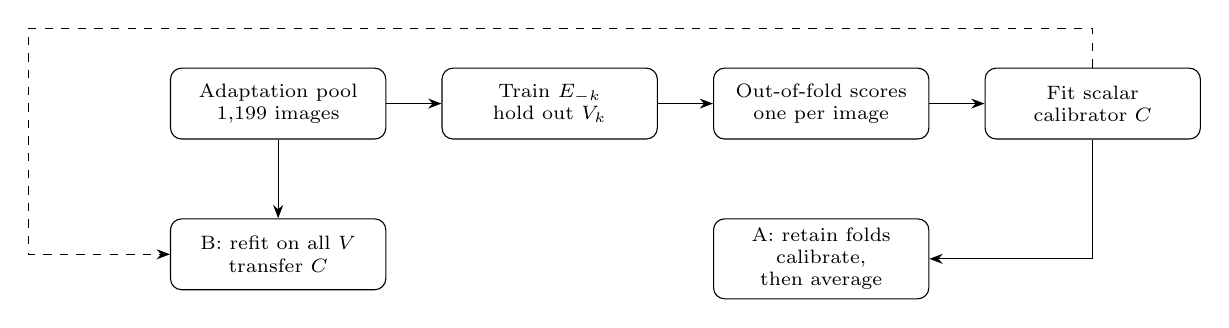
\begin{tikzpicture}[font=\scriptsize,>=Stealth,
box/.style={draw,rounded corners,align=center,minimum height=9mm,text width=25mm}]
\node[box] (v) {Adaptation pool\\1,199 images};
\node[box,right=7mm of v] (fold) {Train $E_{-k}$\\hold out $V_k$};
\node[box,right=7mm of fold] (oof) {Out-of-fold scores\\one per image};
\node[box,right=7mm of oof] (c) {Fit scalar\\calibrator $C$};
\draw[->] (v)--(fold);\draw[->] (fold)--(oof);\draw[->] (oof)--(c);
\node[box,below=10mm of oof] (a) {A: retain folds\\calibrate, then average};
\node[box,below=10mm of v] (b) {B: refit on all $V$\\transfer $C$};
\draw[->] (c.south) |- (a.east);\draw[->] (v)--(b);
\draw[->,dashed] (c.north) -- ++(0,5mm) -| ([xshift=-18mm]v.west) |- (b.west);
\end{tikzpicture}}
\caption{Protocol sketch. A is represented in the completed records; B is a different, proposed inference procedure. Test data enter only after fits and selection rules are frozen.}
\end{figure}

For a \emph{single} score $s=\operatorname{logit}(q)$ and $a>0$, the calibrated binary decision is $s\geq-b/a$. Thus affine calibration and thresholding induce the same family of decision rules, although their fitting objectives differ. For A, $K^{-1}\sum_k\sigma(a s_k+b)$ generally is not a function only of the average $s_k$. Compare (i) thresholding the uncalibrated fold-average score and (ii) a shared threshold shift applied within each fold, alongside the calibrated fold average. Include $a=1,b=0$ and uncalibrated controls.

Do not fit a full-DPE threshold on its in-sample adaptation predictions and describe it as an equally held-out control. Use out-of-fold scores with the same refit transfer, or a documented disjoint fitting pool. If WGA selects a threshold, group labels are required; report this alongside DFR's annotation budget.


\section{Minimum Figures and Tables}
The final paper needs \textbf{two figures and three tables}. Every display should resolve a research question, not illustrate implementation activity.

\textbf{Figure 1: allocation and inference diagram.} Adapt Sect.~\ref{sec:protocol} to show full-validation uniform DPE, the 720/479 split, and cross-fitting. Label which examples fit prototypes, calibration, and selection. Include only inference procedures actually evaluated.

\textbf{Figure 2: allocation sensitivity and paired changes.} Reuse [R1,R3] to plot P0--P2 for fixed uniform, affine, residual, and dropout configurations, with separate backbone panels. Add a full-validation reference line. A paired-source panel can show the primary practical contrast with its interval. A line must never switch hyperparameters to each partition's test winner.

\begin{figure}[ht]
\centering\input{figures/allocation.tex}
\caption{Example panel regenerated from [R3]: standard-ERM source means for the same fixed procedures across allocations. Affine/residual use average group loss and $\lambda=.1$. Descriptive only; uncertainty is not plotted. The residual is exploratory, not a selected proposed method.}
\label{fig:allocation}
\end{figure}

\textbf{Table 1: protocol and information budget.} Rows: full-validation uniform, fixed-split uniform/learned, fold ensemble, refit variant if evaluated, threshold, DFR. Columns: fitting pool sizes; class/group labels used at each stage; head count; selection rule; additional fit/inference cost. All use the same frozen source within a comparison.

\textbf{Table 2: main practical results.} Both backbone recipes separately: WGA mean/SD, overall accuracy, paired change against full-validation DPE, and source counts. Include threshold and DFR once available. Add all four group accuracies/counts in an adjacent panel or supplementary table. Give source-level ERM$^*$ rows because $n=2$ is too small for a persuasive interval.

\textbf{Table 3: compact ablations and sensitivity.} Group the fixed allocation comparisons, original-head cross-fit uncalibrated/calibrated comparisons, and concise H1/H3 negatives. If space is tight, move H1/H3 and the broad grid to the supplement, keeping the main calibration controls in the paper.

Table~\ref{tab:evidence} is an evidence audit for this outline, not a substitute for the final matched-control table. Reuse canonical per-image exports for paired, group-stratified bootstrap analysis. Preserve the minimum over groups in every replicate. Source and conditional image uncertainty answer different questions; report both with clear conditioning if feasible, and do not count folds, partitions, aliases, or combiner initializations as independent backbones.


\section{Completed Work, Pending Work, and What to Omit}
\subsection{Completed, with Scope Limits}
\begin{itemize}
\item \status{DPE reproduction and H2:} five standard-ERM sources [R1] and two ERM$^*$ sources [R2]. Primary dropout gain is +0.6199 pp over matched uniform; paired source 95\% interval [$-0.0218$, +1.2617] pp includes zero. The gain over full-validation uniform is only +0.2586 pp, descriptively. Plain MLP is not clearly inferior.
\item \status{Allocation/H1/H3/sweep:} [R3] records 5,880 rows, comprising 5,222 distinct predictors and 658 algebraic aliases. This is a broad exploratory grid, not 5,880 independent training runs. Three allocations reuse the same sources. Original-head five-fold cross-fitting is completed; full-data refit transfer is not established.
\item \status{Other methods:} AutoBackSwap has useful test evidence but a partial-reproduction status and differing training/information settings [R4]. POTER has a verified selected validation checkpoint, 90.10\% validation WGA and 91.60\% validation overall accuracy; test evaluation remains unverified [R5].
\end{itemize}

\subsection{Minimum Essential Remaining Work, in Order}
\begin{enumerate}
\item \textbf{Freeze the claim and audit existing cross-fit artifacts.} Recover fold assignments, training/held-out image IDs, checkpoint-selection inputs, OOF scores, slopes/offsets, source hashes, and prediction exports. Verify each calibration example is absent from its generating head fit/selection. Inspect the history of the reported +0.47 figure and residual configuration. The current source code and tracked summaries support the documented procedure but are not an independent raw-OOF replay for this outline.
\item \textbf{Finish threshold controls on cached scores.} Use a prespecified score, objective, deterministic tie rule, and the same OOF/disjoint allocation as calibration. Evaluate original heads first, separating the fold-uniform gain from calibration. Avoid another temperature/architecture sweep.
\item \textbf{Run same-feature DFR.} Follow a cited DFR recipe on these frozen features, with validation-only regularization selection and documented group-balanced fitting. Keep feature normalization inside selection folds when learned. Refit after selection and report actual sample/group-label budgets and repeated subsampling. No new backbone training is required.
\item \textbf{Regenerate the final reporting bundle.} For fixed declared procedures, export per-source WGA, OA, four group accuracies/counts, paired changes and uncertainty, plus fit/inference overhead. Use both recipes and all available sources; do not count within-source repeats as new evidence.
\end{enumerate}

\subsection{Conditional Extension and Optional Work}
The proposed full-data-refit calibrator is essential only if the paper claims that particular adaptation. Prioritize the existing five-fold study and controls; attempt refit transfer only after the minimum comparison is secure. Do not launch three- versus five-fold tuning under the deadline. Omit new backbones, more nonlinear gates, species relabeling, expanded prototype sweeps, a full POTER rerun, rotation/fusion screenshots, and causal background interventions from the critical path. A causal claim would require a controlled foreground-preserving intervention and its own controls; current WGA evidence cannot substitute.


\section{Novelty, Rejection Risks, and Submission Decision}
\begin{description}
\item[Incremental novelty.] A combination of established techniques with a small mean gain is a weak method contribution. The feasible response is a focused allocation study with controls that reveal when extra adaptation machinery helps, and when it does not. Novelty is still modest and acceptance cannot be presumed.
\item[Missing simple controls.] A reviewer can reasonably attribute a single-score affine result to threshold movement, or a cross-fit result to extra heads. Complete those controls before claiming an improvement. Same-feature DFR establishes whether the added prototype machinery is practically justified.
\item[Test-informed development.] The brief reports favorable residual selection after examining test WGA. The run documentation states fixed procedures were fitted before test scoring, but that does not rule out later test-informed emphasis. Treat the historical study as exploratory and disclose both facts. A new validation-only selection rerun improves procedure discipline; it does not restore an untouched test set.
\item[Reproduction and protocol mismatch.] The standard-ERM DPE gap remains unresolved; full-data and split methods differ in pool sizes and training updates. Inspect existing preprocessing, checkpoint, scaling, normalization, and update records. If unresolved, report the gap and bound conclusions to the maintained implementation. ERM$^*$ agreement does not validate standard ERM automatically.
\item[Limited precision and scope.] Five/two sources on one repeatedly inspected benchmark cannot establish a broad robustness advance. Show paired differences, uncertainty, and the two ERM$^*$ source values. Additional datasets would strengthen generalization but are outside the current time budget.
\item[Unsupported mechanism.] Improved WGA does not show that backgrounds matter less, that certain heads are causally background-biased, or that apparently unusual species labels are annotation errors. Make performance and allocation claims only.
\end{description}

\textbf{Full-paper decision.} Pursue a full empirical paper only if the artifact audit, matched threshold/DFR controls, and a coherent analysis of allocation/backbone sensitivity are complete. Be explicit if the controls eliminate the apparent methodological advantage. A full empirical paper need not outperform every baseline, but it needs an insight stronger than reproduction plus a sweep. If only unstable gains and incomplete controls remain, prefer a narrower poster/empirical submission or defer; a poster still requires a sound contribution and complete reporting.

\textbf{Remaining-time order (elapsed time from restart).} First 2 hours: artifact audit and fixed protocol. Next 3--4 hours: threshold/DFR fits using caches, while drafting introduction/setup from verified records. Next 2 hours: metrics, uncertainty, tables, and the full-paper decision. Reserve the final 4--5 hours for manuscript assembly, citations, PDF inspection, and submission checks. These are work priorities, not runtime guarantees; stop optional experiments if they threaten a finished, defensible document.


\section{Conference Checks and Evidence Ledger}
The official ACIIDS pages checked on 14 November 2026 specify English Springer LNCS/LNAI PDF submissions, normally 12--15 pages including figures, tables, and references; up to 25 pages may incur extra charges \cite{aciids-submit}. Full papers are associated with LNAI and poster papers with CCIS. The page does not provide a separate shorter poster limit; confirm the selected track's requirements in EasyChair instead of assuming one.

The official dates page states a hard submission deadline of \textbf{14 November 2026, 23:59 AoE}, equivalent to \textbf{15 November 2026, 18:59 Vietnam time} \cite{aciids-dates}. Check the portal's active deadline and any track-specific review/anonymization instructions before uploading. The public submission page inspected does not establish a double-blind requirement. This outline preserves the existing author block for internal use; it is not an instruction to submit an identified manuscript to a blind track.

\subsection{Repository Sources and Recomputed Values}
\noindent\textbf{[R1] Five-source verification.} Protocol, uncertainty, full-validation controls, and allocation sensitivity:
\pathref{results/dpe/five_seed_verification_20261112/README.md}
\pathref{results/dpe/five_seed_verification_20261112/uncertainty.json}
\noindent\textbf{[R2] ERM$^*$ neural aggregation.} Two-source means, selection and recipe details:
\pathref{results/dpe/ermstar_neural_two_seed_20261113/README.md}
\noindent\textbf{[R3] Independent-methods study.} Full/split/fold results and implementation:
\pathref{results/dpe/independent_methods_20261113/{README.md,per_seed.csv,summary.csv}}
\pathref{src/methods/dpe_independent/{README.md,runner.py,fitting.py}}
\noindent\textbf{[R4] AutoBackSwap context and limits.}
\pathref{results/autobackswap/summary_report.md}
\noindent\textbf{[R5] POTER validation-only audit.}
\pathref{results/poter/report.md}
\noindent\textbf{[R6] Historical reports and project protocol.}
\pathref{report/week01/main.tex; report/week02/main.tex}
\pathref{docs/research_protocol.md; docs/methods.md}

Table~\ref{tab:evidence} and Fig.~\ref{fig:allocation} are regenerated by the accompanying \path{build_evidence.py} from [R3]'s source rows. The script verifies WGA against the four group accuracies and recomputed means/sample SDs against tracked summaries. It writes \path{evidence_audit.json}, including paired per-source contrasts. This is a numerical table check, not an independent rerun of historical backbone inference or training. [R1]'s published intervals are used only for its exact matched contrast. No interval is inferred from rounded means, and no unverified result is promoted to a completed experiment.

\begin{thebibliography}{9}
\bibitem{dpe} To, N.N.M., et al.: Diverse Prototypical Ensembles Improve Robustness to Subpopulation Shift. In: ICML, PMLR 267, pp. 59761--59783 (2025). \url{https://proceedings.mlr.press/v267/to25a.html}
\bibitem{waterbirds} Sagawa, S., Koh, P.W., Hashimoto, T.B., Liang, P.: Distributionally Robust Neural Networks for Group Shifts: On the Importance of Regularization for Worst-Case Generalization. ICLR (2020). \url{https://arxiv.org/abs/1911.08731}
\bibitem{dfr} Kirichenko, P., Izmailov, P., Wilson, A.G.: Last Layer Re-Training is Sufficient for Robustness to Spurious Correlations. ICLR (2023). \url{https://arxiv.org/abs/2204.02937}
\bibitem{features} Izmailov, P., Kirichenko, P., Gruver, N., Wilson, A.G.: On Feature Learning in the Presence of Spurious Correlations. NeurIPS 35 (2022). \url{https://arxiv.org/abs/2210.11369}
\bibitem{stacking} Wolpert, D.H.: Stacked generalization. Neural Networks 5(2), 241--259 (1992). \url{https://doi.org/10.1016/S0893-6080(05)80023-1}
\bibitem{calibration} Guo, C., Pleiss, G., Sun, Y., Weinberger, K.Q.: On Calibration of Modern Neural Networks. ICML, PMLR 70, pp. 1321--1330 (2017). \url{https://proceedings.mlr.press/v70/guo17a.html}
\bibitem{aciids-submit} ACIIDS 2027: Submission Guidelines (accessed 14 November 2026). \url{https://aciids.pwr.edu.pl/2027/submit.html}
\bibitem{aciids-dates} ACIIDS 2027: Important Dates (accessed 14 November 2026). \url{https://aciids.pwr.edu.pl/2027/dates.html}
\end{thebibliography}
\end{document}
